\documentclass[conference]{IEEEtran}
\IEEEoverridecommandlockouts
% The preceding line is only needed to identify funding in the first footnote. If that is unneeded, please comment it out.
\usepackage{cite}
\usepackage{amsmath,amssymb,amsfonts}
\usepackage{algorithmic}
\usepackage{graphicx}
\usepackage{textcomp}
\usepackage{xcolor}
\documentclass{article}
\usepackage{tabularx}
\usepackage{colortbl}


\def\BibTeX{{\rm B\kern-.05em{\sc i\kern-.025em b}\kern-.08em
    T\kern-.1667em\lower.7ex\hbox{E}\kern-.125emX}}
\begin{document}

\title{Traffic Sign Recognition With Audio Alert
\\
{\footnotesize \textsuperscript{*}}
\thanks{Identify applicable funding agency here. If none, delete this.}
}

\author{\IEEEauthorblockN{1\textsuperscript{st} Jeet Pankajkumar Parekh}
\IEEEauthorblockA{\textit{Dept.of Applied Data Science } \\
jeetpankajkumar.parekh@sjsu.edu}
\and
\IEEEauthorblockN{2\textsuperscript{nd} Lakshmi Satvika Nekkanti}
\IEEEauthorblockA{\textit{Dept.of Applied Data Science} \\
lakshmisatvika.nekkanti@sjsu.edu}
\and
\IEEEauthorblockN{3\textsuperscript{rd} Sally Wei}
\IEEEauthorblockA{\textit{Dept.of Applied Data Science} \\
sally.wei@sjsu.edu}
\and
 \IEEEauthorblockN{4\textsuperscript{th} Shashidhar Reddy Repala}
\IEEEauthorblockA{\textit{Dept.of Applied Data Science} \\
shashidharreddy.repala@sjsu.edu}
}

\maketitle

\begin{abstract}
Road accidents are becoming more common as a result of increased traffic.Traffic sign awareness is an important step in improving safety and adhering to traffic rules. Additionally, in this project, text to speech conversion is performed by using ppytsx3 library where it gives the output as audio and can be useful for the partially impaired.A German traffic sign dataset with over 40,000 photos of traffic signs are used.This project presents three models: AlexNet, Vgg-19, and CNN.The system's efficiency is noteworthy, with an execution accuracy of approximately 98.52 percent, VGG with and accuracy of 90 percent and alex net with an accuracy of 97.4 percent.
\end{abstract}

\begin{IEEEkeywords}
CNN,AlexNet,VGG-19,ppytsx3,Traffic recognition,Gtsrb
\end{IEEEkeywords}

\section{Introduction}
\subsection{BACKGROUND}
Enhancing road safety through precisely categorizing traffic signs is a pressing concern in today's global context, addressing the most considerable societal need for reduced traffic-related incidents. The harrowing statistics of road accidents and fatalities worldwide punctuate this need. As autonomous vehicles become increasingly commonplace, the necessity for an automatic traffic sign classification system has never been more critical. Such technology can substantially improve fuel efficiency, decrease traffic snarls, and diminish the propensity of accidents induced by driver errors. Beyond these broader safety advantages, a highly accurate traffic sign classification system dramatically improves transportation for individuals grappling with visual impairments or other disabilities that complicate their comprehension of traffic signage, making journeys safer and more accessible.

\subsection{MOTIVATION}
Traffic sign recognition is an integral part of driving safely. With the advent of self-driving systems and driver assistance systems, it becomes more important than ever before to have models that can quickly, accurately, and reliably identify traffic signs using minimal resources and in real time under a variety of circumstances. Current challenges include reliable recognition of traffic signs under difficult weather conditions, such as heavy fog and precipitation, which obstruct vision and greatly increase the chance of a driver missing a traffic sign, which is dangerous and can lead to accidents. Traffic sign recognition systems can assist drivers in reading signs that would otherwise have been missed, increasing safety on the road and improving compliance with posted signs. In addition, such recognition systems are also included in self-driving architectures, which need to be able to identify and recognize traffic signs in real-time.

The reliable classification of traffic signs constitutes a critical aspect with far-reaching ramifications in transportation and driver security. By offering a coherent and precise categorization of traffic signs, potential accidents can be mitigated, traffic flow can be optimized, and drivers can benefit from essential, real-time information. The advent of self-driving cars has further amplified the need for an automated system of traffic sign classification to ensure the safety of occupants and other road users by enabling these vehicles to identify and sort traffic signs with precision. The use of deep learning methodologies and Convolutional Neural Networks (CNNs) can considerably enhance the efficacy and accuracy of this task. The performance of such a traffic sign categorization model could be further enriched by applying transfer learning strategies, such as fine-tuning, thereby leveraging pre-trained layers on large-scale datasets like ImageNet. Incorporating depth data into the classification algorithm by employing RGB-D images is also poised to yield greater robustness and precision outcomes.



\section{LITERATURE REVIEW}

[3]  Noted that there was a major limitation of a lack of sufficient training data for traffic signs under different lighting and weather conditions. They attempted to remedy this by augmenting existing data with synthetic data generated through a DCGAN, and though it did improve the performance of the models they tested it on, the method was computationally expensive, and they only trained their model to generate images of prohibition signs such as stop signs and no entry signs. In comparison, our training set of 43 classes of traffic signs included but was not limited to prohibition signs, and our dataset contained over 80,000 images, compared to Dewi et. al. who were working with 250 images total.

[2] Road signs stand as silent sentinels, their importance unquestionable in maintaining an uninterrupted traffic flow, guarding against the perilous stranglehold of bottlenecks and mishaps. They offer a language in themselves, their pictorial codes weaving narratives of caution and direction, critical for every driver to comprehend. However, it is concerning that these signs, standing tall right in front of our vehicles, often blend into the backdrop of our vision, their messages lost to carelessness. Disregarding these signs can invite disaster, their unheard warnings transforming into tragic accidents. Our study focuses on this issue, comprehensively analyzing traffic sign board detection and recognition. It details an innovative procedure for singling out a road sign from the intricate tapestry of a raw image, interpreting its symbol, and issuing an alert to the driver via a voice command. This mechanism supports the drivers and makes decision-making on the road easier. This companion empathizes with humans and enhances their abilities. It was designed to assist, not replace them.

[1] One of the leading factors contributing to vehicular mishaps is the inadvertent overlooking of roadside signage, coupled with a consequential disregard for road regulations. An innovative signboard detection mechanism within vehicles has been proposed to combat this widespread issue. This cutting-edge system, leveraging the prowess of openCV, is programmed to detect and extract data from signboards. It subsequently alerts the driver via visual cues on a designated LCD screen and auditory prompts relayed through in-car speakers. The ability to recognize and heed traffic signs is vital to the transport infrastructure, particularly on highways or busy roads. This proactive system holds immense potential, capable of playing an instrumental role in preserving countless lives and providing a safety net to lapses in human attention.Other strategies focus on reducing runtime or comparing the performance of different models. [4] trained their dataset on the popular object-detection framework YOLO, which is itself based on convolutional neural networks (CNN), while [6] applied spike neural networks (SNN) to the problem. However, Xie et. al noted that although their SNN produced accurate results with low energy requirements, the model itself formed a black box and could not be easily explained. Additionally, the YOLO model produced by Shivayogi et al. produced a model that had relatively poor accuracy of only around 50-70%, due to their efforts to reduce the complexity of the model.
In summary, it is challenging to make accurate predictions while keeping the model lightweight and when possibly dealing with a lack of diverse training data. Therefore we will work with established lightweight architectures to find one that can predict signs in varying weather conditions accurately.


\section{METHODOLOGY}
\subsection{DATA COLLECTION}
The first challenge was selecting a dataset that had both sufficient size and good diversity of signs. We also wanted a dataset that either contained signs globally across the world, or alternatively a dataset that was confined to a single country, while still accommodating the first two requirements. This was to prevent a sparsity of signs in any one category from being spread too thin across countries.The German Traffic Sign Benchmarks Dataset was used, which contains approximately 43 categories and 40,000 images of traffic signs. 
The data needed to be used with multiple models, so we had to design a processing pipeline that could flexibly account for each of the models to be built. To make collaboration easier while designing the pipeline, the data processing was entirely performed through python and python packages, simplifying the requirements and reducing the number of moving parts. Different versions of data were version controlled on GitHub for management.

\begin{figure}[htp]
    \centering
    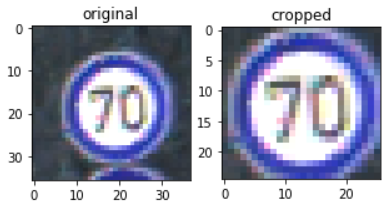
\includegraphics[width=4cm]{images/Screenshot 2023-05-22 104652.png}
    \caption{Resizing Sample}
    \label{fig:galaxy}
\end{figure}
\subsection{DATA PREPROCESSING}\label{AA}
For consistency across models,and to reduce the computational expenses and increase the training speed , the process of data preprocessing commenced with the extraction of traffic sign images from a particular directory, subsequently resizing each to a uniform dimension of 30x30 pixels. 
Transitioning these images into numpy arrays created a more conducive environment for executing deep learning operations. The dataset was split into two main parts: image data, referred to as 'data,' and their respective identifiers, termed 'labels.' These elements were preserved as numpy arrays, thus streamlining their utilization in future endeavors. The entirety of the dataset was then dissected into training and testing subsets, allocating a fifth of the data for testing purposes. Furthermore, the labels were subjected to one-hot encoding, morphing into a categorically graphic format. A final step ensured the data's soundness by diligently managing any exceptions that might arise during the image loading stage.

During the evaluation of model performance, salient indicators such as the time taken for training and testing and metrics of accuracy and loss were considered. We leverage the potency of pre-trained models like VGG19, AlexNet and developed a custom Convolutional Neural Network (CNN) model.Fine-tuning, a superior technique in transfer learning,was applied where the last layers of these models are retrained while the preceding layers are held constant. This strategy tailors the pre-trained models to our specific objective - the classification of traffic signs. Furthermore, to bolster the robustness and precision of the traffic sign classification models, we incorporate depth information derived from RGB images. Utilizing advanced deep learning frameworks such as TensorFlow and PyTorch, we execute the implementation and assessment of the models. The models are evaluated against a specific test set to ascertain their adaptability to unseen data, thereby measuring their potential to generalize effectively.

The final models were integrated into a single python program that managed downloading the dataset, training, testing, and displaying the results of each model. The program and thus each integrated model were version controlled on GitHub, allowing an archive of each model's various versions throughout development.A single Model class implemented shared actions like calculating loss and accuracy, batching data, and saving the model, training history, and performance charts to file. Each individual model's architecture was defined in its own function in the Model class, allowing the Model class to flexibly use any of the models implemented. Each model's individual files are loaded and saved to their own subfolder, to simplify managing the various downloaded and saved files for each version of each model.The details of the training and design of each model are described in detail in the following sections.

\subsection{MODELS DETAILS AND TRAINING}
CNN -In our pursuit of an effective solution for traffic sign classification, a custom Convolutional Neural Network (CNN) model was crafted. The construct of the CNN architecture was carried out through the functional capabilities of the Keras library. The model's design incorporated multiple Conv2D layers that were purposefully established for feature extraction, while MaxPool2D layers facilitated the downsampling process. Additionally, Dense layers were integrated for the final phase of classification. In order to avoid overfitting, Dropout layers were strategically applied as a regularization method. The softmax activation function was invoked within the Dense highest layer, paving the way for the derivation of class probabilities. Subsequently, the model was compiled, employing the categorical cross-entropy loss function in tandem with the Adam optimizer.

Our custom CNN model underwent rigorous training over the course of 15 epochs, utilizing a comprehensive training set. A meticulous record of accuracy and loss values for each epoch was maintained throughout this stage, permitting close scrutiny of the training process. The model's performance was subsequently evaluated on the testing set, employing the evaluation method as a tool for assessment. Crucial evaluation metrics, such as test loss and accuracy, were computed and documented. As part of the evaluation process, two distinct visual representations were designed: a line plot encapsulating training and validation accuracy and another depicting the corresponding loss values, thus providing an illustrative overview of the model's development and efficacy.
\begin{figure}[htp]
    \centering
    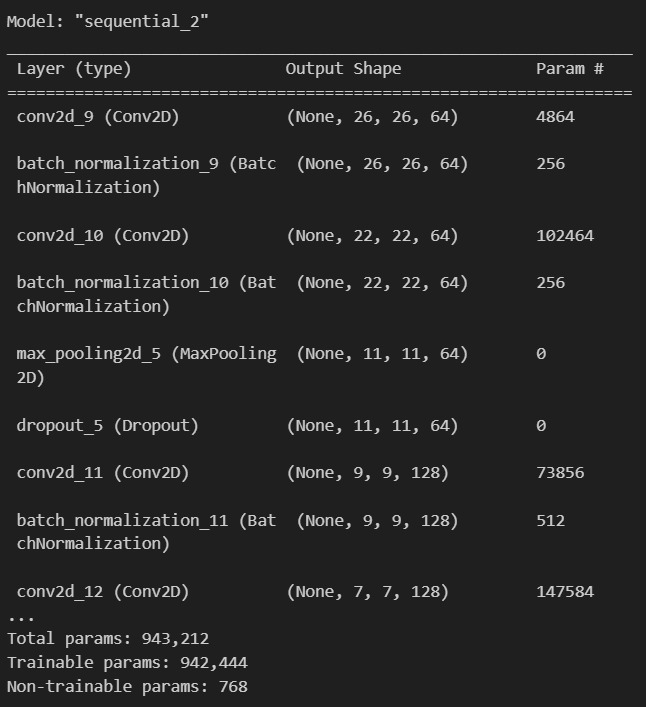
\includegraphics[width=7cm]{images/WhatsApp Image 2023-05-22 at 3.34.52 PM.jpeg}
    \caption{Resizing Sample}
    \label{fig:CNN MOdel Architecture}
\end{figure}
VGG19 - VGG19, short for Visual Geometry Group 19, is  a deep convolutional neural network (CNN) model that is developed by the Visual Geometry Group at the University of Oxford.It has 19 weight layers consisting of 16 convolutional layers with 3 fully connected layers and the same 5 pooling layers. The convolutional layers are configured with small 3x3 filters and a stride of 1 pixel, along with max-pooling layers with 2x2 filters and a stride of 2 pixels, which helps to reduce the spatial dimensions of the feature maps.The pre-processing layer takes the RGB image with pixel values in the range 0 to 255 and subtracts the mean image values computed over the entire ImageNet training collection. After preprocessing, the input images are passed through layers of weight. The training images are processed through a stack of convolutional layers. 
The initial layers capture low-level features such as edges and textures, while the deeper layers learn more complex and abstract features. During training, the model learns to classify images by adjusting the weights of its layers through a process called backpropagation. The weights are updated iteratively using optimization algorithms like stochastic gradient descent, aiming to minimize the difference between the predicted labels and the ground truth labels.

AlexNet architecture consists of eight layers out of which five are convolutional layers and the other three are fully connected layers. This architecture also has three max pooling layers which are not considered as layers in most cases as they don't have any learnable parameters. It uses relu,softmax activation functions. One main advantage of having alexnet is it has dropout layers in the fully connected layer where it saves the model from overfitting of the data and randomly ignores the neurons for better learning and generalization of the features . Alex net was initially trained on 227,227 pixels but for this project it’s being trained on30,30 pixels where the parameters are changed accordingly.The number of strides,kernel filter,and other parameters in normalization layers.In this project alex net had an input shape of 30,30 pixels with batch normalization after every convolutional layer to reduce the distribution of layer inputs as they keep updating. By doing this the model is more stable and also it trains faster. After first,second,fifth convolutional layers there are max pool layers.Two dropout layers with value 0.5 are present.The training accuracy ,validation accuracies are calculated.
 

\section{EVALUATION METRICS}
This project has a total of three models which are,Custom CNN,AlexNet,VGG 19 for which the plots of training loss and accuracy, training time, and testing accuracy determine the accuracy and training speed of each model and each of their versions. All of the models were trained on the same set of data and splits of data, and for the same number of epochs. The total number of epochs were 15,batch size of 32, optimizer was adam.In simple terms Training accuracy measures the accurately predicted values by total images in the train set.Training Loss measures the difference between the ground truth and the predicted value.Validation loss result talks about how well the model is generalizing on the data that it does not see. validation accuracy  measures the accurately predicted values by total images in the validation set.explanation :The training accuracy and validation accuracy were compared. The training loss and validation loss were compared. Additionally f1 score,Precision ,Recall metrics are also evaluated. Next part will cover all the above discussed metrics for all the three models.
The developed system leverages a Convolutional Neural Network (CNN) for Traffic Sign Board Recognition and Voice Alert. This proficient system can detect, recognize, and interpret road traffic signs, offering significant assistance to drivers. The overarching aim is to automate the road sign recognition process, enabling the system to identify and classify traffic signs within live color images.

\section{RESULTS}
The developed system leverages a Convolutional Neural Network (CNN) for Traffic Sign Board Recognition and Voice Alert. This proficient system can detect, recognize, and interpret road traffic signs, offering significant assistance to drivers. The overarching aim is to automate the road sign recognition process, enabling the system to identify and classify traffic signs within live color images.

Our system alerts drivers through voice alerts when it detects signboards. The system empowers the driver to make the necessary corrective decisions to mitigate or avoid an impending incident by providing real-time information from road signs and issuing timely acoustic warnings of potential hazards.
In terms of performance, the proposed system boasts an impressive 98 percent accuracy rate, surpassing other models that was examined. Our model prompts the user with a "No Sign Detected" alert if an image does not contain a traffic sign. Despite the occasional missed detections, the system performs remarkably well, even in complex scenarios. This performance extends to full-resolution images, where all traffic-sign detections are displayed. This indicates that our system provides an efficient deep network for learning numerous categories with effective and swift detection.

We used Python with Flask as our web framework on the Windows operating system. We compiled and applied the model using the fit function, setting the batch size to 32. The graphs depicting the model's accuracy and loss display an average validation accuracy of 98.6 percent and an average training accuracy of 99.3 percent.

Including a voice alert system powered by the pyttsx3 library enhances the usability of our system. This text-to-speech conversion library operates offline and is compatible with Python 2 and 3. The application, by invoking the pyttsx3.init() factory function, provides access to a pyttsx3. Engine instance, thus facilitating easy conversion of entered text into speech. This library supports two male and female voices provided by "sapi5" for Windows.

\subsection{ACCURACY AND LOSS}
In our study, the Convolutional Neural Network (CNN) model was trained over fifteen iterations, culminating in a validation accuracy of 98.6. The validation accuracy plateaued post the eighth epoch, suggesting that additional training might yield slight improvement.

On the other hand, the Alexnet model, after being trained for 15 epochs, demonstrated a training accuracy of 97.80 and a validation accuracy of 97.40. In contrast,the VGG19 model showed a lower final validation accuracy of 90.07 after its 15-epoch training. This inferior accuracy hints at the potential inadequacy of this architecture for the task at hand.The topologies interconnectivity may contribute to feature reuse and a reduced parameter count necessary for a specific performance level.
\begin{figure}[htp]
    \centering
    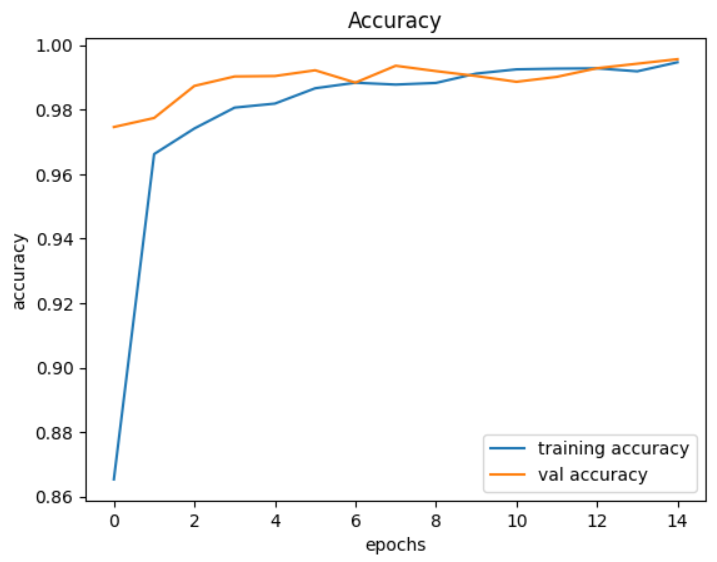
\includegraphics[width=7cm]{images/Accuarcy.png}
    \label{fig:Accuracy}
    \centering
    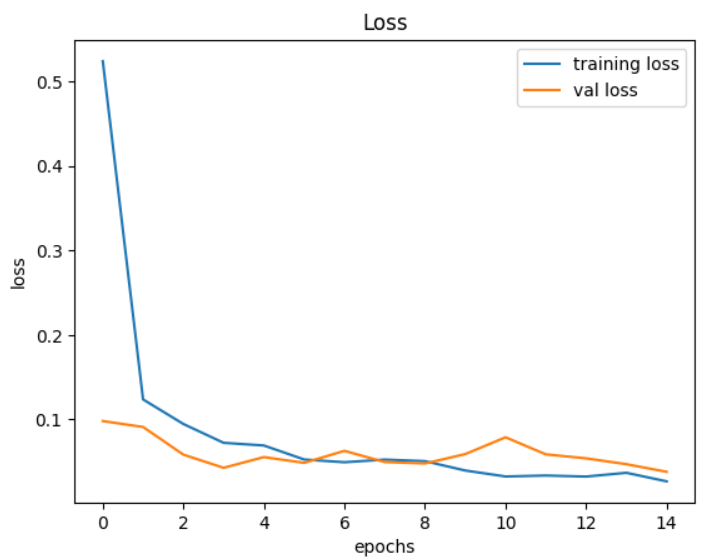
\includegraphics[width=7cm]{images/loss.png}
    \caption{CNN-Accuracy vs Loss for 15 epochs}
    \label{fig:Loss}
\end{figure}

The final step involved incorporating a customized layer, a more fitting solution for this classification problem. Concurrently, the model's loss function visibly decreased as the model's predictive accuracy improved on the training data. An under-fitting scenario is apparent towards the end of the training, given that the validation loss starts to decline in the concluding two epochs.
\begin{table}
\caption{Performance Metrics }
\begin{center}
\begin{tabular}{||c c c c||} 
\hline
Model & F1 Score & Precision & Recall \\ [0.5ex] 
\hline\hline
CNN & 0.995 & 0.995 & 0.995 \\ 
\hline
VGG19 & 0.923 & 0.948 & 0.899 \\
\hline
Alex Net & 0.975 & 0.982 & 0.968 \\
\hline
\end{tabular}
\end{center}
\end{table}
\subsection{Web Application}
The web application utilizes Flask, a Python web framework, to recognize and interpret traffic signs in real time. Users can upload an image using the application of a traffic sign, which the program then processes and classifies using a pre-trained Convolutional Neural Network (CNN) model. A total of 44 different traffic signs are recognized by the system, each having a unique identifier. Upon receiving an image, the program resizes it to a 30x30 pixel resolution, converts it into a NumPy array, and feeds it into the model for prediction. The model then returns the class with the highest predicted probability.
    \begin{figure}[htp]
    \centering
    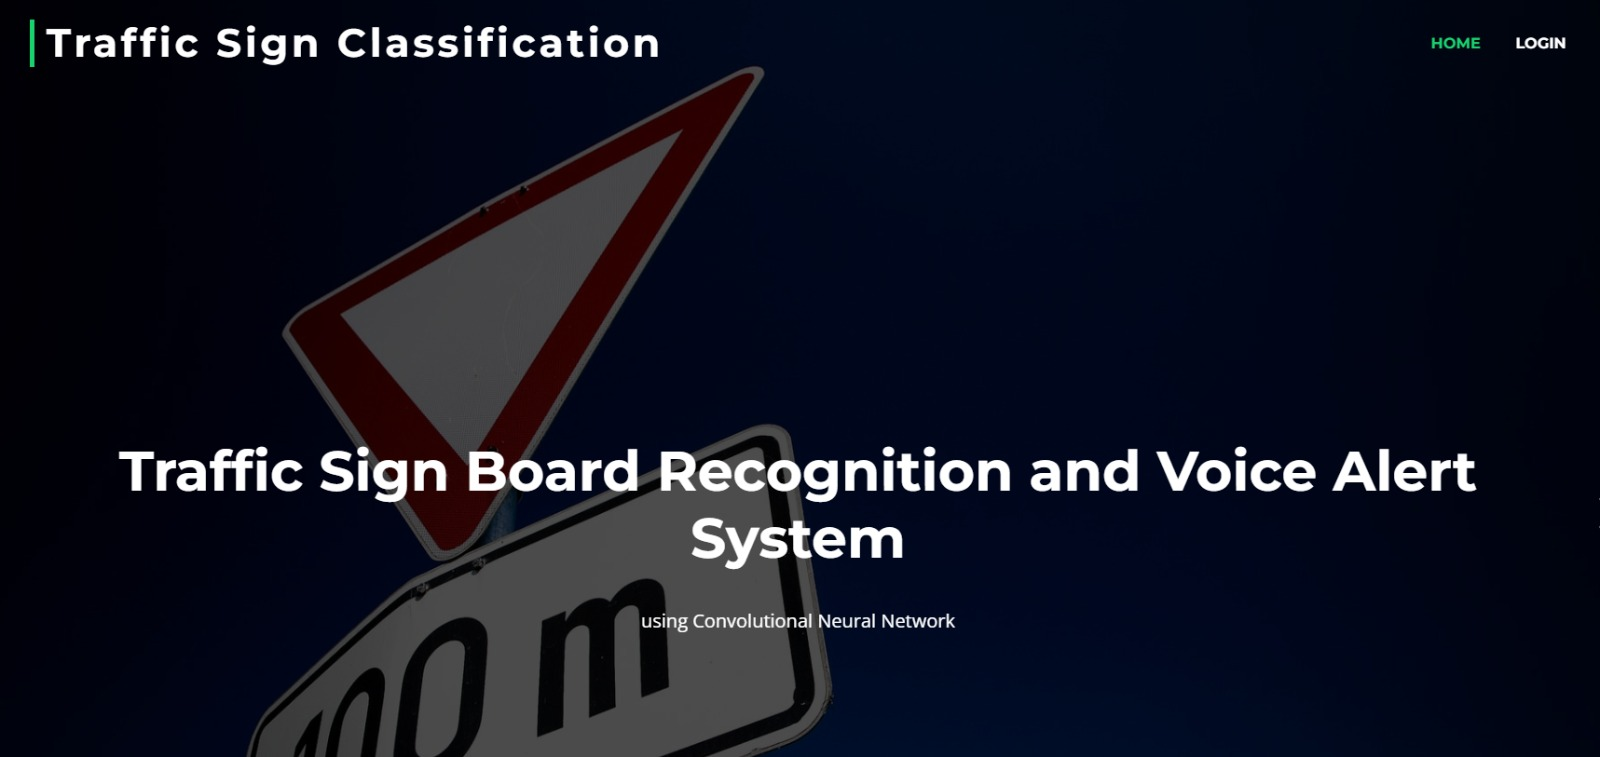
\includegraphics[width=7cm]{images/predict.jpeg}
    \centering
    \caption{GUI Homepage}
    \end{figure}
  \begin{figure}[htp]
    \centering
    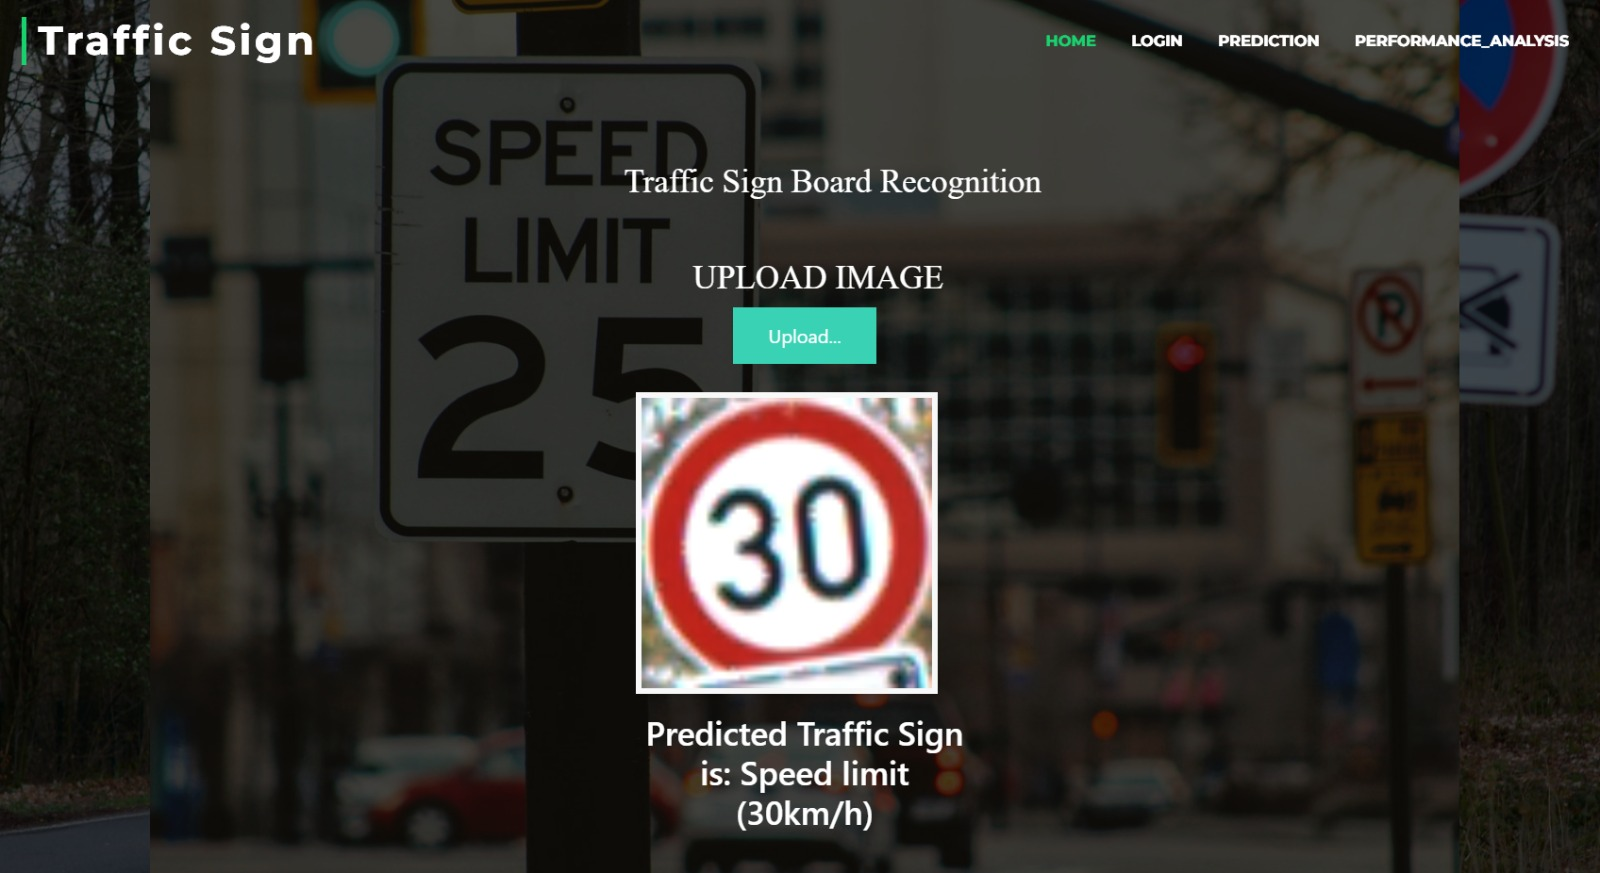
\includegraphics[width=7cm]{images/GUI.jpeg}
    \centering
    \caption{UI to upload Image and predict the sign}
    \end{figure}
The focus is on the user-friendly interface facilitated by our Flask application. The app features several routes or endpoints, such as index, login, and performance, each corresponding to a specific HTML template that renders upon access. For instance, the login route leads to a login page, while the performance route showcases the model's performance. The main feature, however, is the 'predict' endpoint. Upon accessing this route, users can upload an image file of a traffic sign, which the system classifies. After predicting the traffic sign, the application deletes the uploaded file for data security, generates a voice alert using the pyttsx3 library that reads out the prediction, and then returns the result to the user. In essence, this web application enhances the usability of the traffic sign recognition system, making it accessible to any user with a standard web browser.
    
\subsection{Command Line Interface}
A command-line interface allows users to download the data, split the data, train each of the models, and display training result information all in one place. It also handles downloading existing models or training history, as well as downloading existing splits for the data. The program is written completely in Python using Python libraries. It consists of four files: the main file, main.py, containing the main program entry and general logic; Models.py which contains shared code for displaying information related to each model, as well as the individual architectures for each model; CustomArgParser.py which parses the arguments for the program and defines its help command; and Globals.py which is a configuration file containing static information like file locations and file download URLs. The graphical user interface is also archived with the rest of the code as trainapp.py.
\begin{figure}[htp]
    \centering
    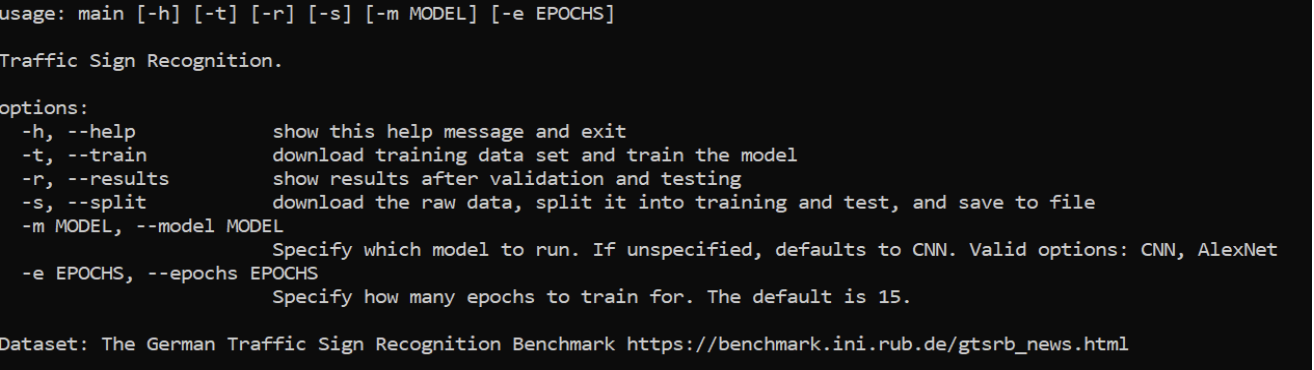
\includegraphics[width=7cm]{images/CLI.png}
    \centering
    \caption{Help Command For Command-line Interface}
    \end{figure}
\subsection{Discussion}
The proposed methodology encompasses the development of a Traffic Sign Board Recognition and Voice Alert System underpinned by Convolutional Neural Networks (CNN). This advanced system can detect, discern, and interpret traffic signs, significantly aiding the driver. The automated road sign recognition system, the linchpin of our proposal, is specifically designed to detect and categorize various road signs in real-time color images. Upon successful sign detection, the system ensures driver alertness by vocalizing the details of the detected sign. This real-time road sign information relay forms the crux of our system, as it can pre-emptively issue an acoustic warning, allowing the driver to react suitably to potential hazards.

Most existing research pertains to the automatic detection and recognition of symbol-based traffic signs or text identification in real-world scenarios. However, the focus on recognizing text on traffic information signs could be improved. Moreover, deep learning's application to a broad set of traffic-sign categories is needed without an extensive dataset featuring several hundred categories, each with an adequate number of instances. In addition, many current systems focus more on traffic-sign recognition (TSR) and may not adequately address the more challenging task of traffic-sign detection (TSD).In this area, pinpointing an accurate sign location is paramount. Additionally, detecting numerous other traffic-sign classes not included in existing benchmarks poses significant challenges due to their high appearance variation.
The proposed system has an impressive accuracy rate of 97, which is better than the existing models we evaluated. A built-in feature also alerts the user with a "No Sign Detected" prompt if an image does not contain a traffic sign. The system has demonstrated commendable performance, handling complex cases exceptionally well despite occasionally missed detections. Its robustness is further reflected in its ability to display all traffic-sign detections for several full-resolution images. Ultimately, the proposed system provides an efficient deep network for learning many categories, offering swift and accurate detection. 
\section{FUTURE SCOPE}
In smart cities and autonomous vehicles, traffic sign recognition is pivotal. A well-implemented strategy can enhance the effectiveness of these systems by improving the accuracy of traffic sign classification. Future enhancements could include comparing performance across various neural networks, adding more layers to the model, tuning hyperparameters, and using data augmentation techniques. Moreover, maintaining ethical standards like privacy and transparency is crucial in responsible AI deployment. We plan to expand our dataset to include worldwide data and incorporate multi-language voice output for broader accessibility. Ultimately, these advancements promise improved traffic safety and responsible utilization of AI technologies.
\begin{figure}[htbp]
\caption{ TEAM CONTRIBUTION}
\centering
\begin{minipage}{0.5\textwidth}
\renewcommand{\arraystretch}{1.2} % Adjust row height
\setlength{\tabcolsep}{3pt} % Adjust column spacing (reduced from 6pt)
\arrayrulecolor{black} % Set line color to black
\begin{tabularx}{\linewidth}{|>{\raggedright\arraybackslash}X|>{\raggedright\arraybackslash}p{4cm}|}
\hline
\rowcolor{black!10} % Set background color for header row
\textbf{Name} & \textbf{Tasks} \\ \hline
Jeet Pankajkumar Parekh & Worked on custom CNN and web app. \\
Lakshmi Satvika Nekkanti & Tested and trained AlexNet and pyttsx3. \\
Sally Wei & Created CLI and worked on GitHub. \\
Shashidhar Reddy Repala & Helped with dataset preprocessing, trained and tested VGG19. \\
\hline
\end{tabularx}
\end{minipage}
\end{figure}


\begin{thebibliography}{00}
\bibitem{b1} Anushree.A., S., Kumar, H., Iram, I., and Divyam, K.(2019). Automatic Signboard Detection System by the Vehicles.
\bibitem{b2} Harini, S., Abhiram, V. P., Hegde, R., Samarth, B. D. D., Shreyas, S. A., and Gowranga, K. H. (2017). A smart driver alert system for vehicle traffic using image detection and recognition technique. 
\bibitem{b3} Dewi, C., Chen R.C., Liu Y.T., Tai S.K (2021). Synthetic Data generation using DCGAN for improved traffic sign recognition. Neural Computing and Applications, 34, 21465–21480. https://doi.org/10.1007/s00521-021-05982-z
\bibitem{b4} Shivayogi1, A.B., Dharmendra1, N.C.M, Ramakrishna, A.M., and Subramanya, K.N. (2022). Real-Time Traffic Sign Recognition Using Deep Learning. Pertanika Journal of Science and Technology, 31(1), 137-148. https://doi.org/10.47836/pjst.31.1.09
\bibitem{b5} Sukhani, K., Shankarmani, R., Shah, J., Shah, K. (2021). Traffic Sign Board Recognition and Voice Alert System using Convolutional Neural Network. . IEEE Conference Publication | IEEE Xplore. https://ieeexplore.ieee.org/document/9456302
\bibitem{b6} Xie, K., Zhang, Z., Li, B., Yu, R., Niyato, D., Xie, S., and Wu, Y. (2022). Efficient Federated Learning With Spike Neural Networks for Traffic Sign Recognition. IEEE Transactions on Vehicular Technology, 71(9), 9980–9992. https://doi.org/10.1109/tvt.2022.317880 
\end{thebibliography}
\vspace{12pt}

\end{document}
